
\documentclass[12pt,a4paper,final]{article}
\usepackage[utf8]{inputenc}
\usepackage[francais]{babel}
\usepackage[T1]{fontenc}
\usepackage{amsmath}
\usepackage{amsfonts}
\usepackage{amsthm}
\usepackage{color}
\usepackage{amssymb}
\usepackage{graphicx}
\usepackage{algorithm}
\usepackage{algorithmic}
\usepackage{fancyhdr}
\usepackage[fs]{umons-coverpage}

%%###### START CHANGE HERE ######
\author{Simon Olbregts}
\title{Plus courts chemins dans un graphe pondéré}
\umonsAuthor{Simon Olbregts}
%% The main title of your thesis
\umonsTitle{Plus courts chemins\\ dans un graphe pondéré}
%% The sub-title of your thesis
\umonsSubtitle{Projet réalisé dans le cadre \\de la 1er Master en Sciences informatique}
%% Your supervisor(s)
\umonsSupervisor{\\Véronique Bruyère}
%% The date (or academic year)
\umonsDate {novembre 2014}
%%###### END CHANGEMENT ######

\newcommand{\smalltitle}[1]{\bigskip\large\textbf{#1}\par\normalsize\medskip}
\newcommand{\partitle}[1]{\bigskip\textit{\underline{#1}}\par\medskip}

\newtheorem{defi}{Définition}
\newtheorem{note}{Note}
\newtheorem{prop}{Propriété}
\newtheorem{exemple}{Exemple}
\newtheorem{corollaire}{Corollaire}
\newtheorem{lemme}{Lemme}
\newtheorem{rem}{Remarque}
\newtheorem{thm}{Théorème}

\fancyhf{}
\chead{\leftmark}
\rfoot{\thepage}

\begin{document}

\umonsCoverPage
\pagebreak

\pagestyle{fancy}

\thispagestyle{empty}
\newpage
\tableofcontents
\newpage

%%###### LE RAPPORT COMMENCE ICI ######
\smalltitle{Note préliminaire}
\addcontentsline{toc}{section}{Note préliminaire}
La rédaction de ce document est basé sur le livre \textit{Introduction to algorithme}~\cite{intro_to_algo}

\section{Introduction}
\subsection{Problème posé}
Quelque exemple d'utilisation. \textit{"Un peu d'italique"} \textbf{Du Gras}. Pour séparer deux paragraphe il suffit de mettre deux enter (une ligne blanche en gros)

Et voila un nouveau paragraphe :)\\
On peut egalement simplement revenir en arriere comme ca \\

Une petite liste a puce ? numéroté?

\begin{itemize}
\item $V$ est un ensemble fini de noeuds
\item $E$ est un ensemble d'arcs reliant deux noeuds
\end{itemize}

\begin{enumerate}
\item Remplacer la valeur de la racine par celle du dernier noeud, celui qui sera le plus à droite de la dernière ligne (le "1" dans l'exemple de la figure~\ref{heapExample}(a)).
\item Supprimer ce dernier noeud
\item Faire redescendre tant que nécessaire la nouvelle racine.
\end{enumerate}
Une image ? Avec une reference dans un texte ? no probleme :p

Un graphe orienté est défini par un couple: $G=(V,E)$.
La figure~\ref{graphExample} illustre un graphe.

\begin{figure}
	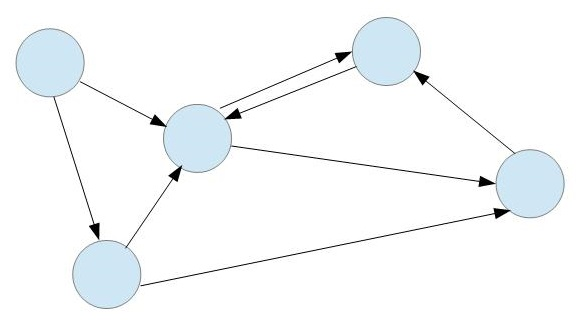
\includegraphics[width=\textwidth]{images/Graph.jpg}
	\caption{\label{graphExample}Exemple de graphe contenant 5 noeuds et 8 arcs}
\end{figure}


La complexité c'est pas un simple O(lg n) mais $\mathcal{O}(\log_2 n)$.\\

\smalltitle{un petit titre qui n'apparait pas dans la table des matiere}
blablabla

\partitle{encore un plus petit titre}
blablabla

Un algorithme ? ouille ouille ouille :p mais on si habitue. Le caption sera le titre visible et le label sera ce que tu devra utiliser pour le referencer comme ca Alogo~\ref{extractMin}

\begin{algorithm}[H]
\caption{extractMin($A$)}\label{extractMin}
\begin{algorithmic}[1]
\STATE $min\gets A[1]$
\STATE $A[1]\gets A[A.heapsize]$
\STATE $A.heapsize\gets A.heapsize - 1$
\STATE heapify($A, 1$)
\end{algorithmic}
\end{algorithm}

\begin{algorithm}[H]
\caption{heapify($A,i$)}\label{heapify}
\begin{algorithmic}[1]
\STATE $l\gets $left($i$)
\STATE $r\gets $right($i$)
\IF{$l \leq A.heapsize$ \AND $A[l] < A[i]$ }
\STATE $smallest\gets l$
\ELSE
\STATE $smallest\gets i$
\ENDIF
\IF{$r <leq A.heapsize$ \AND $A[r] < A[smallest]$}
\STATE $smallest\gets r$
\ENDIF
\IF{$i \neq smallest$}
\STATE switch($A[i], A[smallest]$)
\STATE heapify($A, smallest$)
\ENDIF
\end{algorithmic}
\end{algorithm}

\begin{algorithm}[H]
\caption{decreaseKey($A,i,key$)}\label{heapify}
\begin{algorithmic}[1]
\IF{$key > A[i]$}
\STATE \textbf{error} "la nouvelle clé doit être inférieur à la valeur actuel"
\ENDIF
\STATE $A[i]\gets key$
\WHILE{$i>1$ \AND $A[$parent($i$)$] > A[i]$}
\STATE switch($A[i],A[$parent($i$)$]$)
\STATE $i\gets $parent($i$)
\ENDWHILE
\end{algorithmic}
\end{algorithm}

Des theorme, lemme, propriete ? sa marche aussi :). De nouveaux tu peux reference le label :) Lemme~\ref{upper-bound_prop}

\begin{lemme}[Propriété de borne supérieur]\label{upper-bound_prop}
Nous avons à tout moment $v.d \geq \delta(s,v) \forall v \in V$, et une fois que $v.d$ atteins $\delta(s,v)$ il ne changera plus.
\end{lemme}

\begin{corollaire}[Propriété d'absence de chemin]\label{no_path_prop}
Si il n'existe pas de chemin allant de $s$ à $v$ alors nous avons à tout moment $v.d = \delta(s,v) = \infty$.
\end{corollaire}

\begin{prop}[Propriété de convergence]\label{convergence_prop}
Si $s \leadsto u \rightarrow v$ est un plus court chemin dans $G$ pour $u, v \in V$ donné et si $u.d = \delta(s,u)$ avant que l'arc ($u,v$) ne soit relaxé alors $v.d = \delta(s,v)$ après la relaxation.
\end{prop}

\begin{thm}[Thm de convergence]\label{convergence_thm}
Si $s \leadsto u \rightarrow v$ est un plus court chemin dans $G$ pour $u, v \in V$ donné et si $u.d = \delta(s,u)$ avant que l'arc ($u,v$) ne soit relaxé alors $v.d = \delta(s,v)$ après la relaxation.
\end{thm}

des symbole grec, mathematique $\delta(a), \sigma(a), \neq, \leq, \geq, ...$\\
Ca doit etre entre dollard. Pareil pour toutes les variables, formule, ...\\
on n'ecrit pas l'index i mais l'index $i$

N'oublions pas la bibliographie :)

\bibliographystyle{plain}
\bibliography{reference}

\end{document} 